% RESULTADOS------------------------------------------------------------------

\chapter{RESULTADOS}
\label{chap:resultados}

\par Neste capítulo serão apresentados os resultados obtidos durante o desenvolvimento e as validações do algoritmo proposto neste trabalho de conclusão de curso. De tal forma, os resultados serão apresentados levando em consideração os \textit{datasets} utilizados e apresentados na \autoref{subsec:datasets} e os métodos apresentados na \autoref{sec:metodo}.
\par Além disso, mais detalhes como o relatório de classificação pelas classes dos \textit{datasets}, precisão micro e macro, \textit{recall} micro e macro e \textit{F1-score} micro e macro, estão presentes no repositório do GitHub\footnote{\url{https://github.com/felipeseolin/mst-texture-descriptor-tests}.}.

% Dataset USC-SIPI TEXTURES
\section{USC-SIPI TEXTURES}
\label{sec:uscSipiTextures}

A \autoref{tab:uscSipiAcuracias} apresenta os resultados das acurácias obtidas durantes os testes. É possível observar que utilizando de \textit{Decision Tree} o extrator com melhor acurácia é Gabor (100,0\%), sendo o método proposto o terceiro melhor empatado com LBP e Tamura (78,95\%). Utilizando KNN, os extratores com melhores acurácias são Gabor, Haralick e MST (método proposto), todos com 78,95\%. Ao utilizar \textit{Linear} SVC, o melhor resultado é do extrator LBP (68,42\%), seguido do MST (63,16\%). Por fim, com SVC o extrator com maior acurácia é o proposto (42,11\%).

\begin{table}[H]
    \centering
    \caption[Resultado das acurácias obtidas no \textit{dataset} USC-SIPI \textit{Textures}]{Resultado das acurácias obtidas no \textit{dataset} USC-SIPI \textit{Textures}
    \label{tab:uscSipiAcuracias}}
    \begin{tabular}{rrrrrr}
        \toprule
            & Gabor (\%) & Haralick (\%) & LBP (\%) & Tamura (\%) & MST (\%) \\
        \midrule
            Decision Tree & 100,00 & 89,47 & 78,95 & 78,95 & 78,95 \\
            KNN & 78,95 & 78,95 & 15,79 & 10,53 & 78,95 \\
            Linear SVC & 5,26 & 21,05 & 68,42 & 0,00 & 63,16 \\
            SVC & 21,05 & 36,84 & 10,53 & 0,00 & 42,11 \\
        \bottomrule
    \end{tabular}
    \fonte{Autoria Própria.}
\end{table}


\par As figuras \ref{fig:uscSipiDecisionTreeMatrizConfusao}, \ref{fig:uscSipiKNNMatrizConfusao}, \ref{fig:uscSipiLinearSVCMatrizConfusao} e \ref{fig:uscSipiSVCMatrizConfusao}, expõem e comparam as matrizes de confusão do melhor extrator em relação ao proposto, ou, nos casos em que o MST se destaca como melhor, a sua comparação com o segundo melhor, para cada algoritmo de aprendizado supervisionado utilizado.

\begin{figure}[H]
    \centering
    \caption{Matrizes de confusão para USC-SIPI \textit{Textures dataset} com uso de Decision Tree}
    \subfloat[\centering Gabor]{{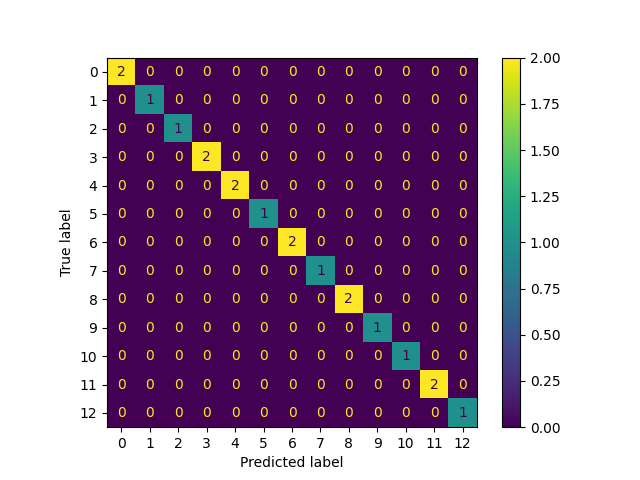
\includegraphics[width=0.45\textwidth]{dados/figuras/resultados/matrizes-confusao/gabor-brodatz-decision-tree.png} }}
    \qquad
    \subfloat[\centering MST]{{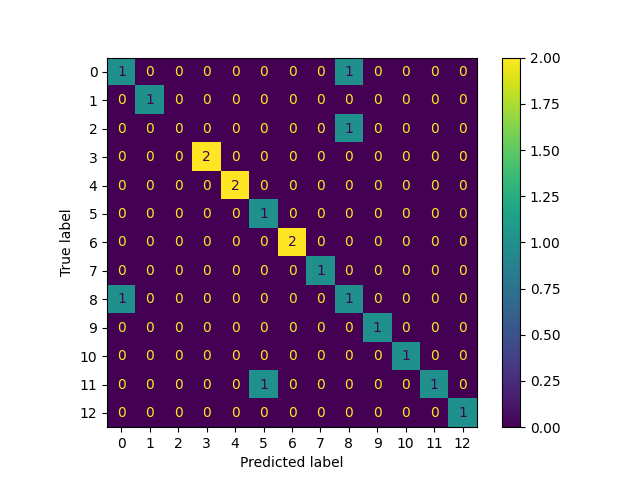
\includegraphics[width=0.45\textwidth]{dados/figuras/resultados/matrizes-confusao/mst-brodatz-decision-tree.png}}}
    \fonte{Autoria Própria.}
    \label{fig:uscSipiDecisionTreeMatrizConfusao}
\end{figure}

\begin{figure}[!h]
    \centering
    \caption{Matrizes de confusão para USC-SIPI \textit{Textures dataset} com uso de KNN}
    \subfloat[\centering Gabor]{{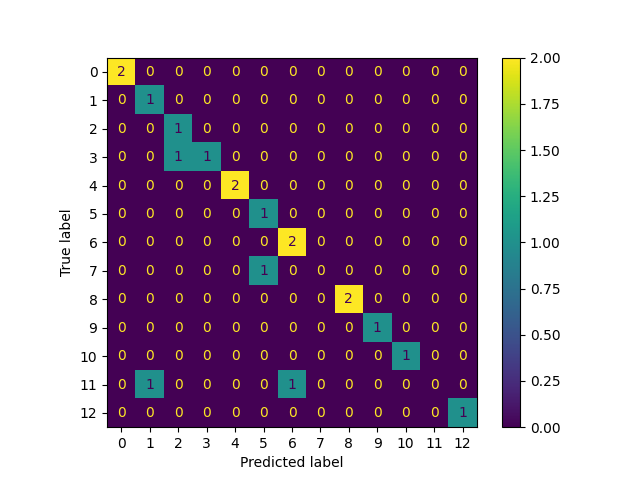
\includegraphics[width=0.45\textwidth]{dados/figuras/resultados/matrizes-confusao/gabor-brodatz-knn.png} }}
    \qquad
    \subfloat[\centering Haralick]{{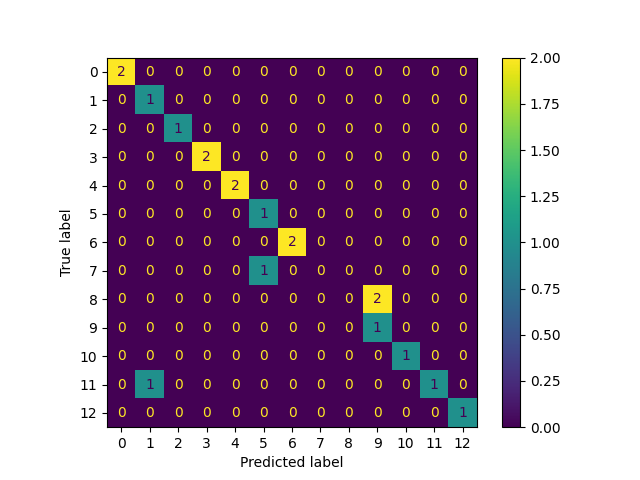
\includegraphics[width=0.45\textwidth]{dados/figuras/resultados/matrizes-confusao/haralick-brodatz-knn.png}}}
    \qquad
    \subfloat[\centering MST]{{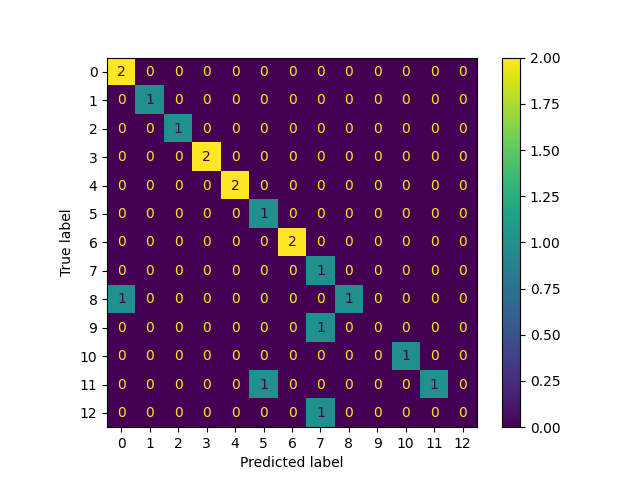
\includegraphics[width=0.45\textwidth]{dados/figuras/resultados/matrizes-confusao/mst-brodatz-knn.png}}}
    \fonte{Autoria Própria.}
    \label{fig:uscSipiKNNMatrizConfusao}
\end{figure}

\begin{figure}[!h]
    \centering
    \caption{Matrizes de confusão para USC-SIPI \textit{Textures dataset} com uso de \textit{Linear} SVC}
    \subfloat[\centering LBP]{{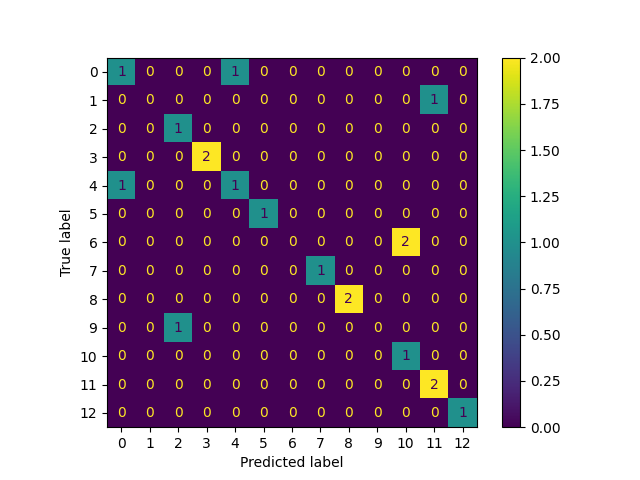
\includegraphics[width=0.45\textwidth]{dados/figuras/resultados/matrizes-confusao/lbp-brodatz-linear-svc.png} }}
    \qquad
    \subfloat[\centering MST]{{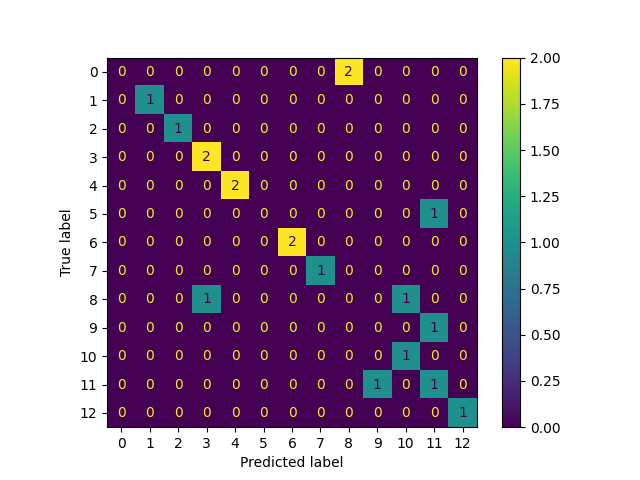
\includegraphics[width=0.45\textwidth]{dados/figuras/resultados/matrizes-confusao/mst-brodatz-linear-svc.png}}}
    \fonte{Autoria Própria.}
    \label{fig:uscSipiLinearSVCMatrizConfusao}
\end{figure}

\begin{figure}[!h]
    \centering
    \caption{Matrizes de confusão para USC-SIPI \textit{Textures dataset} com uso de SVC}
    \subfloat[\centering MST]{{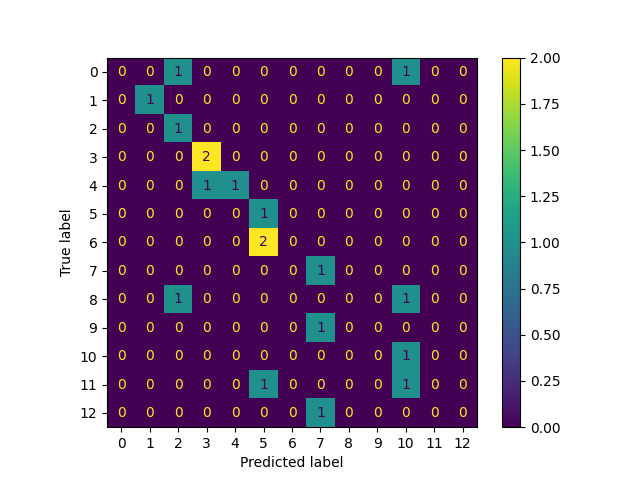
\includegraphics[width=0.45\textwidth]{dados/figuras/resultados/matrizes-confusao/mst-brodatz-svc.png}}}
    \qquad
    \subfloat[\centering Haralick]{{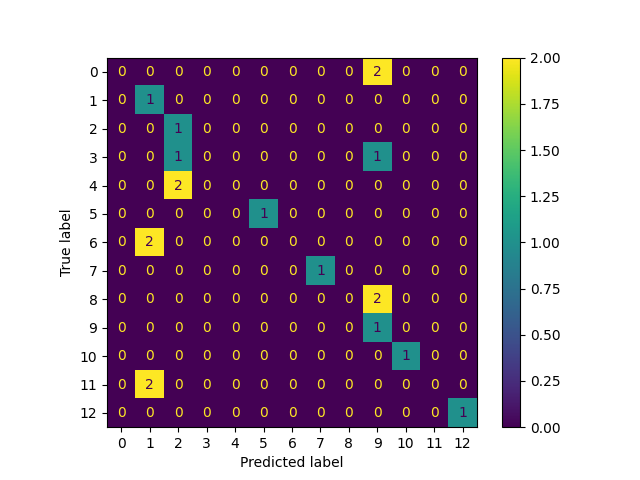
\includegraphics[width=0.45\textwidth]{dados/figuras/resultados/matrizes-confusao/haralick-brodatz-svc.png} }}
    \fonte{Autoria Própria.}
    \label{fig:uscSipiSVCMatrizConfusao}
\end{figure}

% Dataset Kylberg
\section{KYLBERG}
\label{sec:kylberg}

\par A partir dos testes realizados no \textit{dataset} Kylberg, foram estraídas as acurácias que estão disponíveis na \autoref{tab:kylbergAcuracias}. Através dos resultados pode-se observar que com o uso de \textit{Decision Tree} o extrator que obteve a melhor acurácia foi o LBP (93,30\%), seguido pelo Haralick (88,28\%) e pelo extrator proposto (88,06\%), respectivamente. Ao utilizar KNN, o extrator LBP apresentou novamente a melhor acurácia (96,21\%), seguido pelo MST (79,46\%). Com o algoritmo de aprendizado supervisionado \textit{Linear} SVC, o extrator LBP apresentou pela terceira vez o melhor resultado no \textit{dataset} (99,33\%), com o segundo lugar para o MST (68,75\%). Por fim, o SVC apresentou-se como o melhor resultado do extrator LBP (94,08\%), seguido por Tamura (64,17\%) e depois pelo extrator proposto (55,92\%). As matrizes de confusão para a comparação entre as melhores acurácias são expressas nas figuras \ref{fig:kylbergDecisionTreeMatrizConfusao}, \ref{fig:kylbergKNNMatrizConfusao}, \ref{fig:kylbergLinearSVCMatrizConfusao} e \ref{fig:kylbergSVCMatrizConfusao}.

\begin{table}[H]
    \centering
    \caption[Resultado das acurácias obtidas no \textit{dataset} Kylberg]{Resultado das acurácias obtidas no \textit{dataset} Kylberg
    \label{tab:kylbergAcuracias}}
    \begin{tabular}{rrrrrr}
        \toprule
            & Gabor (\%) & Haralick (\%) & LBP (\%) & Tamura (\%) & MST (\%) \\
        \midrule
            Decision Tree & 19,98 & 88,28 & 93,30 & 73,10 & 88,06 \\
            KNN & 18,64 & 46,21 & 96,21 & 59,38 & 79,46 \\
            Linear SVC & 9,71 & 5,69 & 99,33 & 26,34 & 68,75 \\
            SVC & 8,82 & 29,58 & 94,08 & 64,17 & 55,92 \\
        \bottomrule
    \end{tabular}
    \fonte{Autoria Própria.}
\end{table}


\begin{figure}[H]
    \centering
    \caption{Matrizes de confusão para o \textit{dataset} Kylberg com uso de \textit{Decision Tree}}
    \subfloat[\centering LBP]{{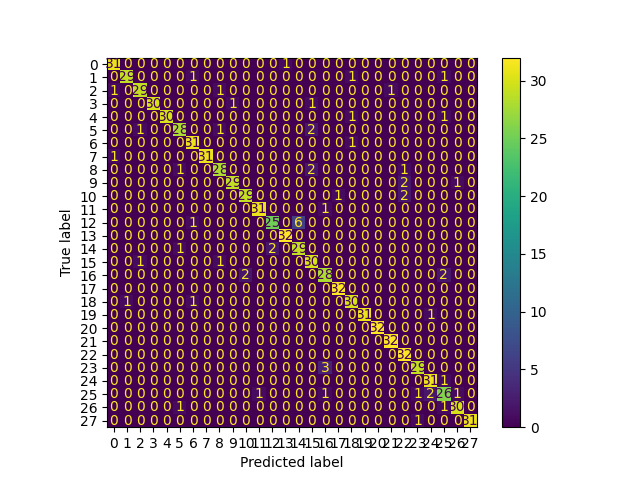
\includegraphics[width=0.45\textwidth]{dados/figuras/resultados/matrizes-confusao/lbp-kylberg-decision-tree.png}}}
    \qquad
    \subfloat[\centering Haralick]{{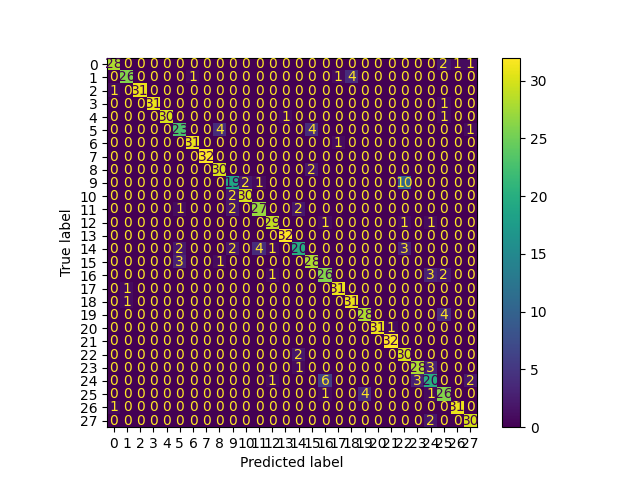
\includegraphics[width=0.45\textwidth]{dados/figuras/resultados/matrizes-confusao/haralick-kylberg-decision-tree.png} }}
    \qquad
    \subfloat[\centering MST]{{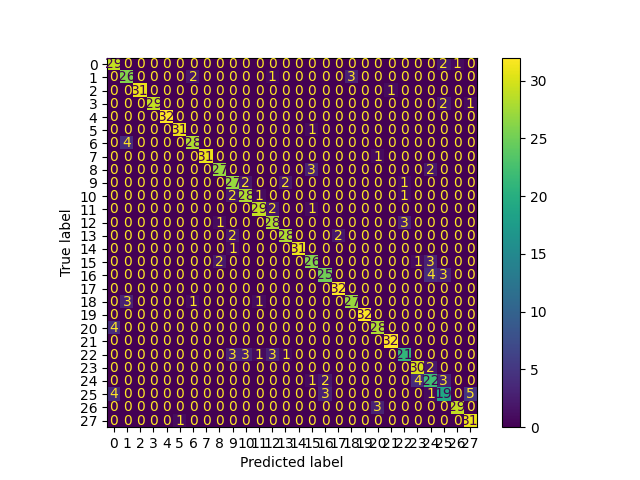
\includegraphics[width=0.45\textwidth]{dados/figuras/resultados/matrizes-confusao/mst-kylberg-decision-tree.png} }}
    \fonte{Autoria Própria.}
    \label{fig:kylbergDecisionTreeMatrizConfusao}
\end{figure}

\begin{figure}[H]
    \centering
    \caption{Matrizes de confusão para o \textit{dataset} Kylberg com uso de KNN}
    \subfloat[\centering LBP]{{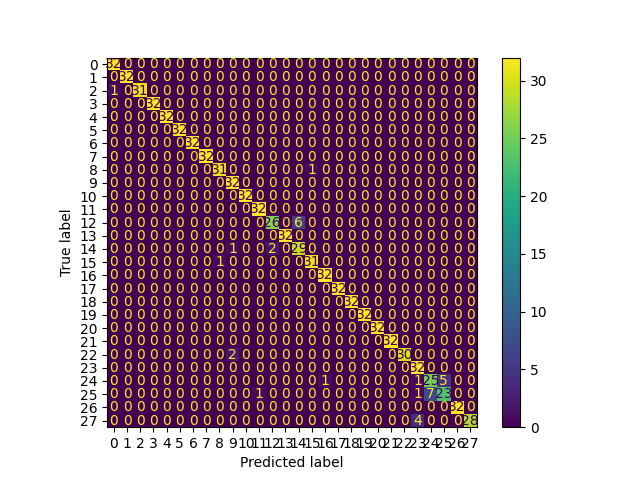
\includegraphics[width=0.45\textwidth]{dados/figuras/resultados/matrizes-confusao/lbp-kylberg-knn.png}}}
    \qquad
    \subfloat[\centering MST]{{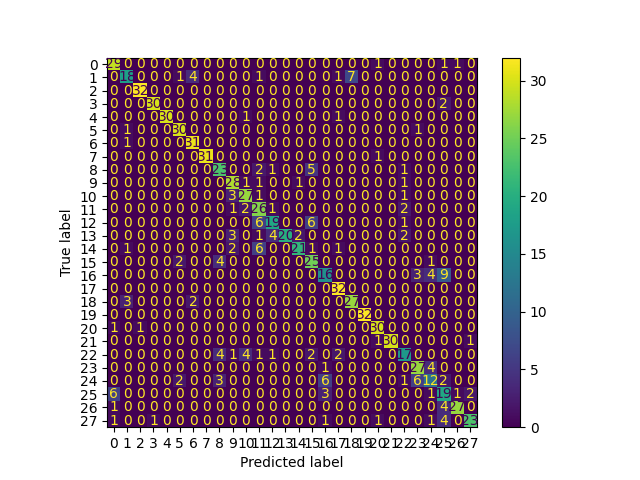
\includegraphics[width=0.45\textwidth]{dados/figuras/resultados/matrizes-confusao/mst-kylberg-knn.png} }}
    \fonte{Autoria Própria.}
    \label{fig:kylbergKNNMatrizConfusao}
\end{figure}


\begin{figure}[H]
    \centering
    \caption{Matrizes de confusão para o \textit{dataset} Kylberg com uso de \textit{Linear} SVC}
    \subfloat[\centering LBP]{{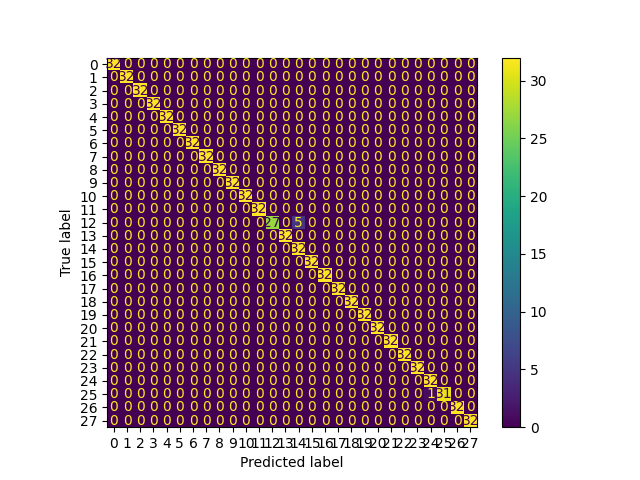
\includegraphics[width=0.45\textwidth]{dados/figuras/resultados/matrizes-confusao/lbp-kylberg-linear-svc.png}}}
    \qquad
    \subfloat[\centering MST]{{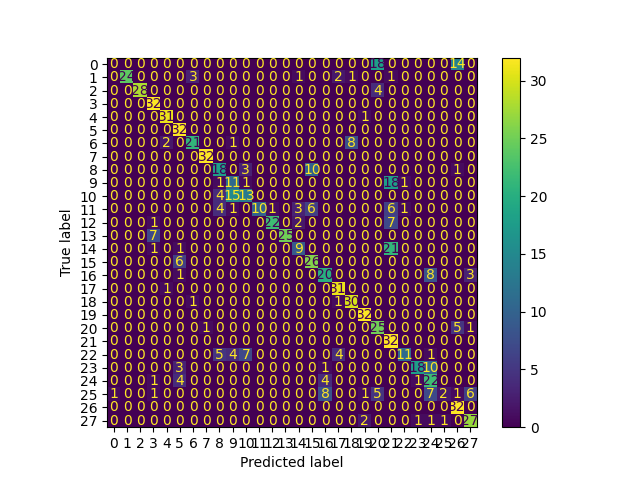
\includegraphics[width=0.45\textwidth]{dados/figuras/resultados/matrizes-confusao/mst-kylberg-linear-svc.png} }}
    \fonte{Autoria Própria.}
    \label{fig:kylbergLinearSVCMatrizConfusao}
\end{figure}

\begin{figure}[H]
    \centering
    \caption{Matrizes de confusão para o \textit{dataset} Kylberg com uso de SVC}
    \subfloat[\centering LBP]{{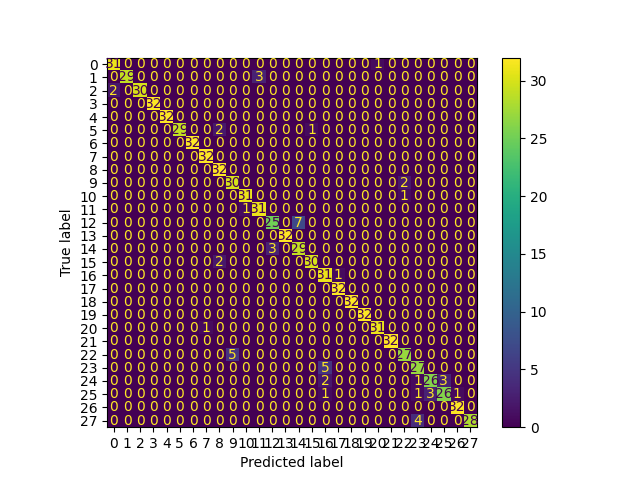
\includegraphics[width=0.45\textwidth]{dados/figuras/resultados/matrizes-confusao/lbp-kylberg-svc.png}}}
    \qquad
    \subfloat[\centering Tamura]{{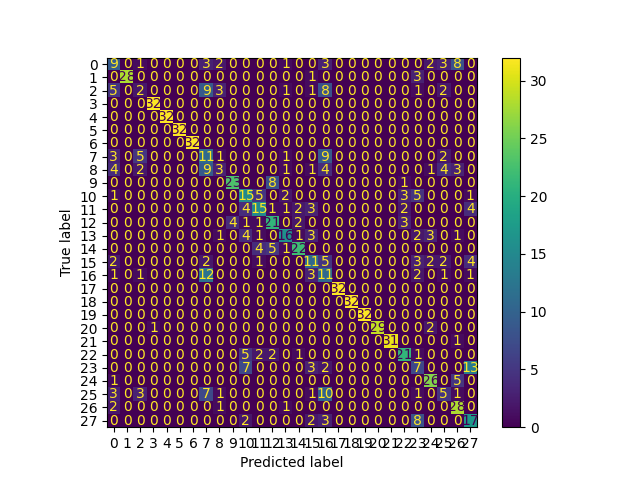
\includegraphics[width=0.45\textwidth]{dados/figuras/resultados/matrizes-confusao/tamura-kylberg-svc.png} }}
    \qquad
    \subfloat[\centering MST]{{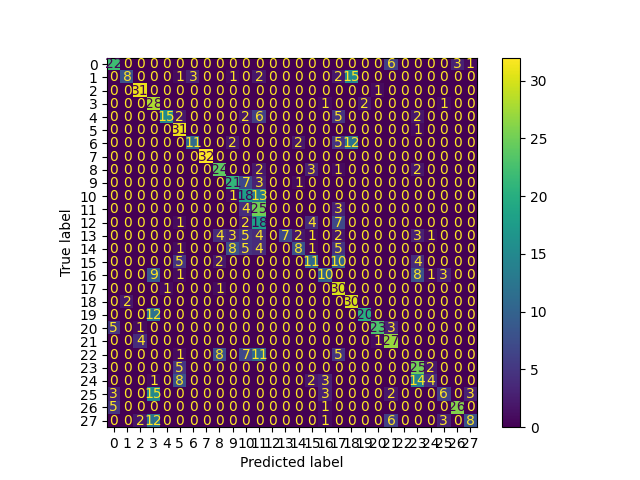
\includegraphics[width=0.45\textwidth]{dados/figuras/resultados/matrizes-confusao/mst-kylberg-svc.png} }}
    \fonte{Autoria Própria.}
    \label{fig:kylbergSVCMatrizConfusao}
\end{figure}

% Dataset USPTex
\section{USPTEX}
\label{sec:usptex}

\par Os resultados das acurácias obtidas para os extratores e algoritmos de aprendizado supervisionado no \textit{dataset} USPtex estão descritos na \autoref{tab:USPtexAcuracias}. Com o Decision Tree, a maior acurácia corresponde ao extrator LBP (44.66\%), estando o algoritmo proposto na quarta posição (31,81\%). Ao utilizar KNN, o melhor extrator é o LBP (77,12\%), seguido do Tamura (30,28\%) e logo após o MST (19,61\%). Já com \textit{Linear} SVC, o melhor resultado se mantém com o extrator LBP (76,47\%), seguido pelo MST (13,51\%). Ao fim, utilizando SVC, o LBP se apresentou com a maior acurácia (46,19\%), após Tamura (24,84\%) e MST (10,24\%). Assim como exemplificado nos \textit{datasets} anteriores, nas figuras \ref{fig:usptexDecisionTreeMatrizConfusao}, \ref{fig:usptexKNNMatrizConfusao}, \ref{fig:usptexLinearSVCMatrizConfusao} e \ref{fig:usptexSVCMatrizConfusao} se encontram as comparações entre matrizes de confusão.

\begin{table}[H]
    \centering
    \caption[Resultado das acurácias obtidas no USPtex]{Resultado das acurácias obtidas no \textit{dataset} USPtex
    \label{tab:USPtexAcuracias}}
    \begin{tabular}{rrrrrr}
        \toprule
            & Gabor (\%) & Haralick (\%) & LBP (\%) & Tamura (\%) & MST (\%) \\
        \midrule
            Decision Tree & 20,92 & 42,05 & 44,66 & 32,90 & 31,81 \\
            KNN & 6,10 & 7,41 & 77,12 & 30,28 & 19,61 \\
            Linear SVC & 1,96 & 1,53 & 76,47 & 8,50 & 13,51 \\
            SVC & 6,10 & 6,10 & 46,19 & 24,84 & 10,24 \\
        \bottomrule
    \end{tabular}
    \fonte{Autoria Própria.}
\end{table}


\begin{figure}[H]
    \centering
    \caption{Matrizes de confusão para o \textit{dataset} USPtex com uso de \textit{Decision Tree}}
    \subfloat[\centering LBP]{{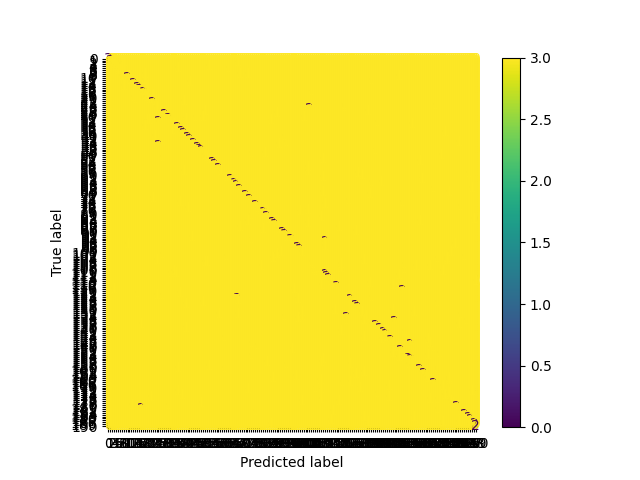
\includegraphics[width=0.45\textwidth]{dados/figuras/resultados/matrizes-confusao/lbp-usptex-decision-tree.png}}}
    \qquad
    \subfloat[\centering Haralick]{{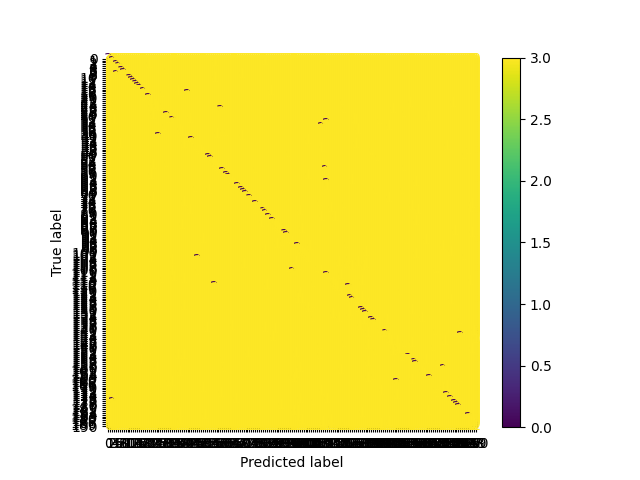
\includegraphics[width=0.45\textwidth]{dados/figuras/resultados/matrizes-confusao/haralick-usptex-decision-tree.png} }}
    \qquad
    \subfloat[\centering Tamura]{{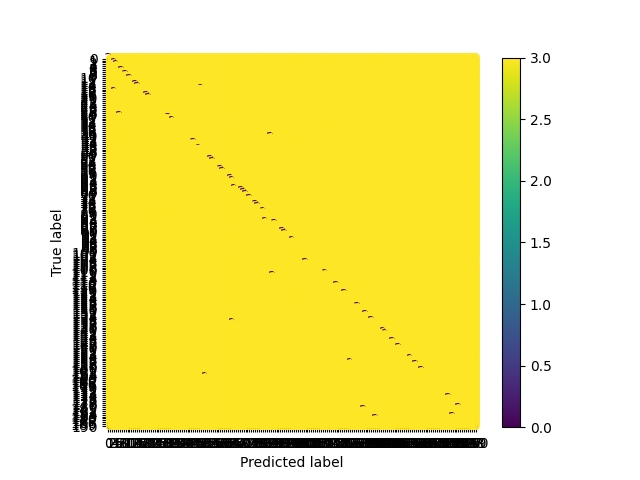
\includegraphics[width=0.45\textwidth]{dados/figuras/resultados/matrizes-confusao/tamura-usptex-decision-tree.png} }}
    \qquad
    \subfloat[\centering MST]{{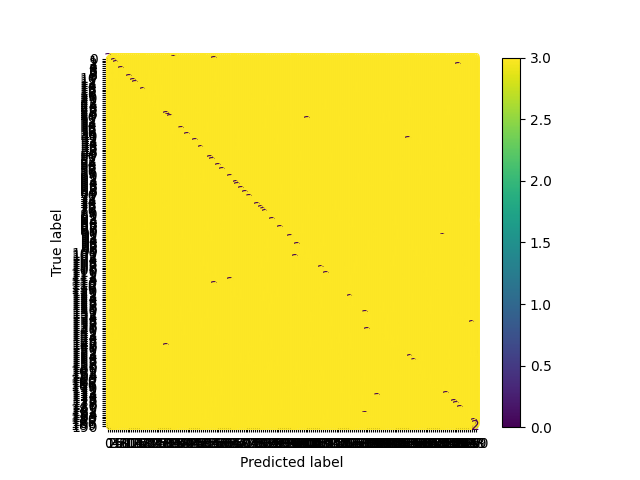
\includegraphics[width=0.45\textwidth]{dados/figuras/resultados/matrizes-confusao/mst-usptex-decision-tree.png} }}
    \fonte{Autoria Própria.}
    \label{fig:usptexDecisionTreeMatrizConfusao}
\end{figure}

\begin{figure}[H]
    \centering
    \caption{Matrizes de confusão para o \textit{dataset} USPtex com uso de KNN}
    \subfloat[\centering LBP]{{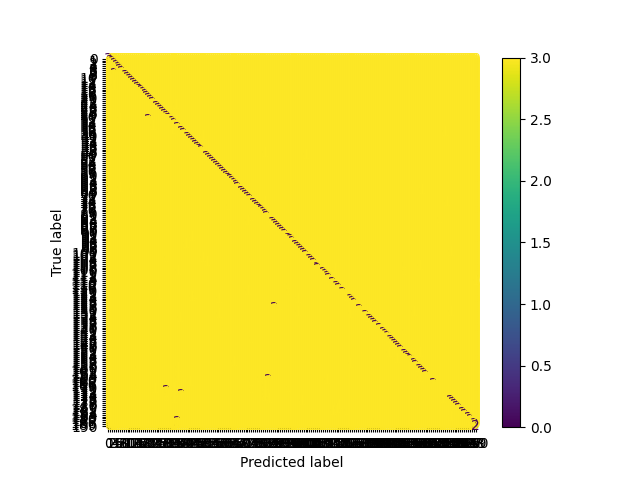
\includegraphics[width=0.45\textwidth]{dados/figuras/resultados/matrizes-confusao/lbp-usptex-knn.png}}}
    \qquad
    \subfloat[\centering Tamura]{{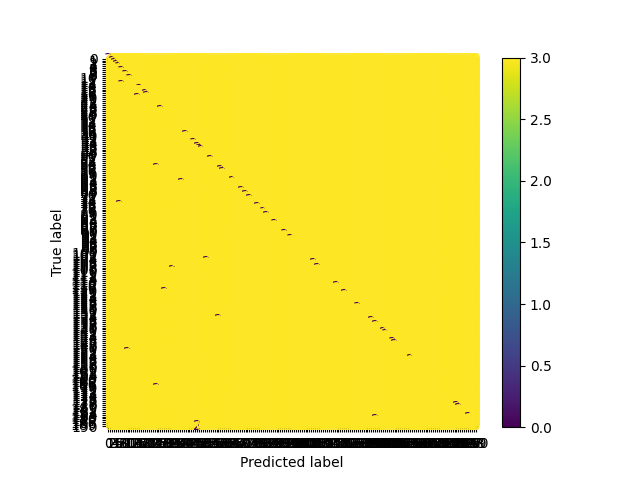
\includegraphics[width=0.45\textwidth]{dados/figuras/resultados/matrizes-confusao/tamura-usptex-knn.png} }}
    \qquad
    \subfloat[\centering MST]{{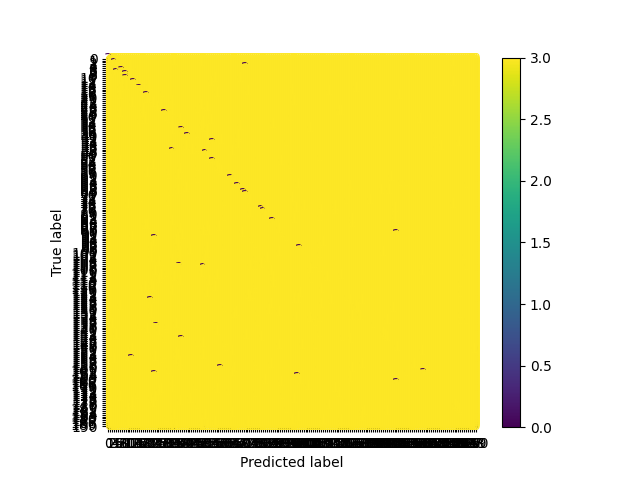
\includegraphics[width=0.45\textwidth]{dados/figuras/resultados/matrizes-confusao/mst-usptex-knn.png} }}
    \fonte{Autoria Própria.}
    \label{fig:usptexKNNMatrizConfusao}
\end{figure}

\begin{figure}[H]
    \centering
    \caption{Matrizes de confusão para o \textit{dataset} USPtex com uso de \textit{Linear} SVC}
    \subfloat[\centering LBP]{{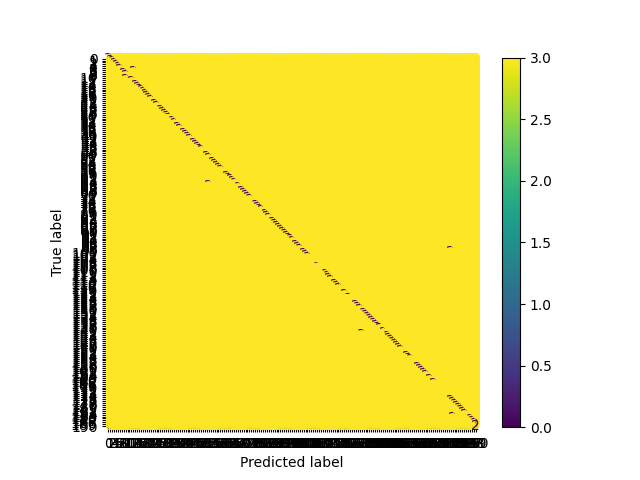
\includegraphics[width=0.45\textwidth]{dados/figuras/resultados/matrizes-confusao/lbp-usptex-linear-svc.png}}}
    \qquad
    \subfloat[\centering MST]{{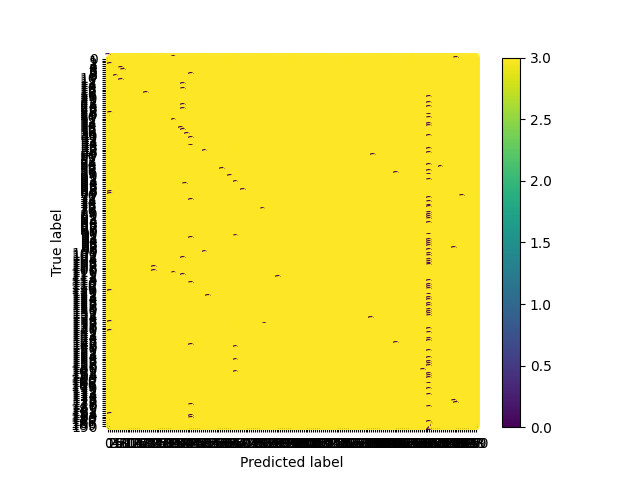
\includegraphics[width=0.45\textwidth]{dados/figuras/resultados/matrizes-confusao/mst-usptex-linear-svc.png} }}
    \fonte{Autoria Própria.}
    \label{fig:usptexLinearSVCMatrizConfusao}
\end{figure}

\begin{figure}[H]
    \centering
    \caption{Matrizes de confusão para o \textit{dataset} USPtex com uso de SVC}
    \subfloat[\centering LBP]{{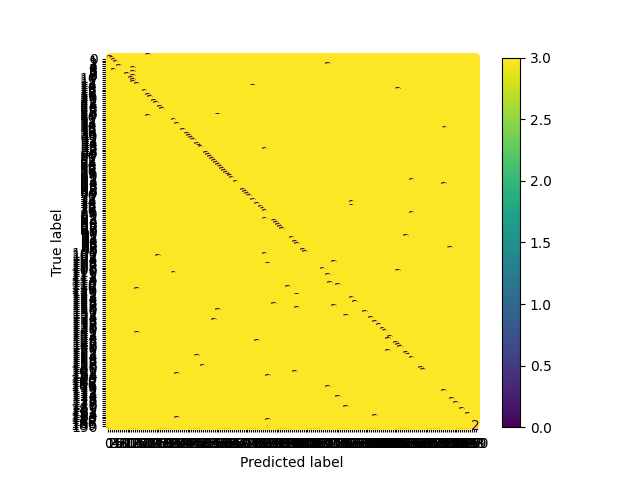
\includegraphics[width=0.45\textwidth]{dados/figuras/resultados/matrizes-confusao/lbp-usptex-svc.png}}}
    \qquad
    \subfloat[\centering Tamura]{{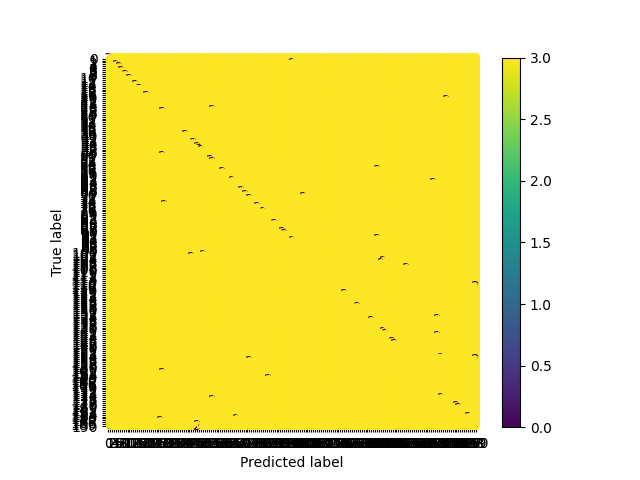
\includegraphics[width=0.45\textwidth]{dados/figuras/resultados/matrizes-confusao/tamura-usptex-svc.png} }}
    \qquad
    \subfloat[\centering MST]{{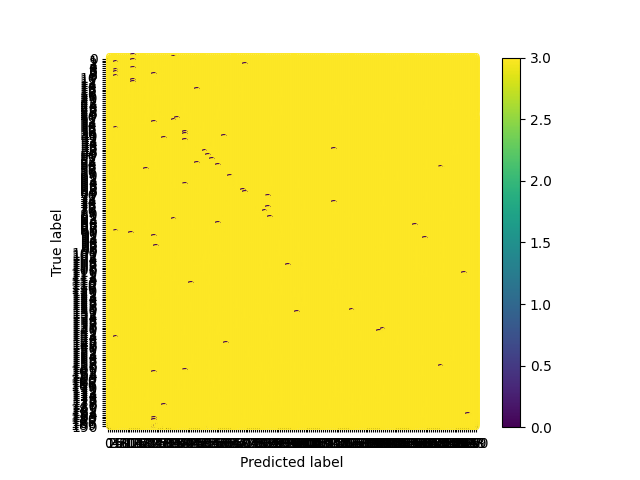
\includegraphics[width=0.45\textwidth]{dados/figuras/resultados/matrizes-confusao/mst-usptex-svc.png} }}
    \fonte{Autoria Própria.}
    \label{fig:usptexSVCMatrizConfusao}
\end{figure}

% Dataset VisTex
\section{VISTEX}
\label{sec:vistex}

\par Por fim, a tabela \autoref{tab:visTexAcuracias} representa uma comparação entre os valores obtidos das acurácias dos testes realizados no \textit{dataset} VisTex. Com o uso de \textit{Decision Tree} a maior acurácia foi do extrator MST (38,24\%), seguido por Gabor (29,41\%). Já o melhor resultado obtido com KNN, foi do extrator LBP, empatado com Tamura (29,41\%), seguido por Haralick que também ficou empatado com o MST (23,53\%). Para \textit{Linear} SVC, a maior acurácia foi do extrator LBP (52,94\%), seguido por Tamura (23,53\%) e posteriormente pelo MST (14,71\%). Para SVC, os extratores Gabor, Haralick e Tamura obtiveram a mesma acurácia de 26,47\%, seguido do LBP (23,53\%) e por fim MST (17,65\%). As figuras \ref{fig:vistexDecisionTreeMatrizConfusao}, \ref{fig:vistexKNNMatrizConfusao}, \ref{fig:vistexLinearSVCMatrizConfusao} e \ref{fig:vistexSVCMatrizConfusao}, exibem as matrizes de confusão obtidas durante os testes com o \textit{dataset} para fins de comparação.

\begin{table}[H]
    \centering
    \caption[Resultado das acurácias obtidas no VisTex]{Resultado das acurácias obtidas no \textit{dataset} VisTex.
    \label{tab:visTexAcuracias}}
    \begin{tabular}{rrrrrr}
        \toprule
            & Gabor (\%) & Haralick (\%) & LBP (\%) & Tamura (\%) & MST (\%) \\
        \midrule
            Decision Tree & 29,41 & 23,53 & 14,71 & 20,59 & 38,20 \\
            KNN & 20,59 & 23,53 & 29,41 & 29,41 & 23,53 \\
            Linear SVC & 11,76 & 5,88 & 52,94 & 23,53 & 14,71 \\
            SVC & 26,47 & 26,47 & 23,53 & 26,47 & 17,65 \\
        \bottomrule
    \end{tabular}
    \fonte{Autoria Própria}
\end{table}


\begin{figure}[H]
    \centering
    \caption{Matrizes de confusão para o \textit{dataset} VisTex com uso de \textit{Decision Tree}}
    \subfloat[\centering MST]{{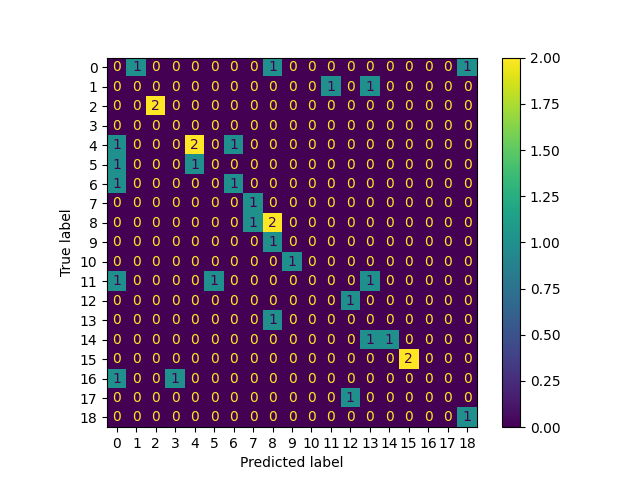
\includegraphics[width=0.45\textwidth]{dados/figuras/resultados/matrizes-confusao/mst-vistex-decision-tree.png} }}
    \qquad
    \subfloat[\centering Gabor]{{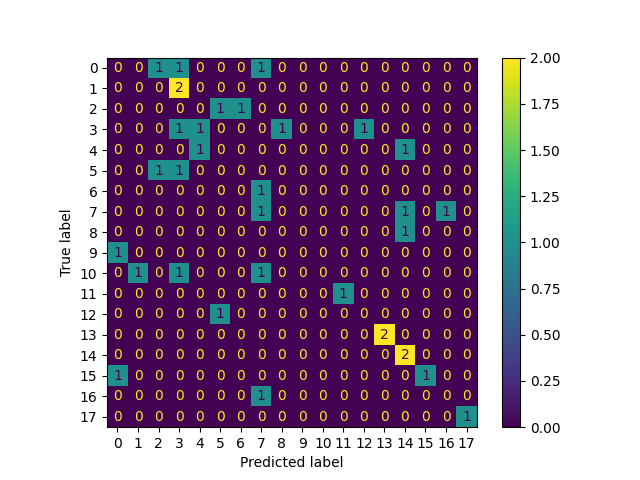
\includegraphics[width=0.45\textwidth]{dados/figuras/resultados/matrizes-confusao/gabor-vistex-decision-tree.png}}}
    \fonte{Autoria Própria.}
    \label{fig:vistexDecisionTreeMatrizConfusao}
\end{figure}

\begin{figure}[H]
    \centering
    \caption{Matrizes de confusão para o \textit{dataset} VisTex com uso de KNN}
    \subfloat[\centering LBP]{{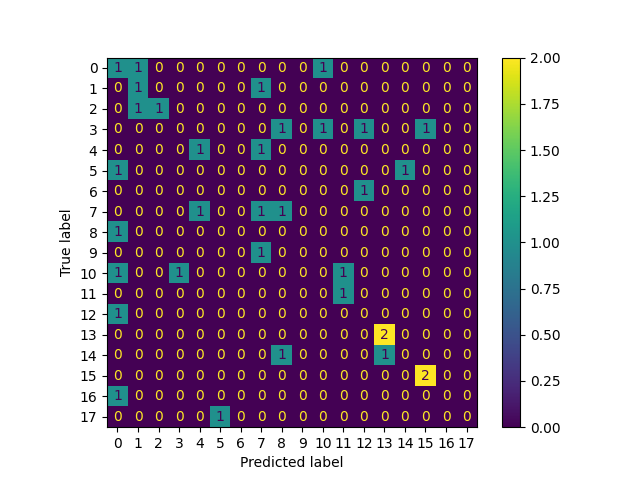
\includegraphics[width=0.45\textwidth]{dados/figuras/resultados/matrizes-confusao/lbp-vistex-knn.png}}}
    \qquad
    \subfloat[\centering Tamura]{{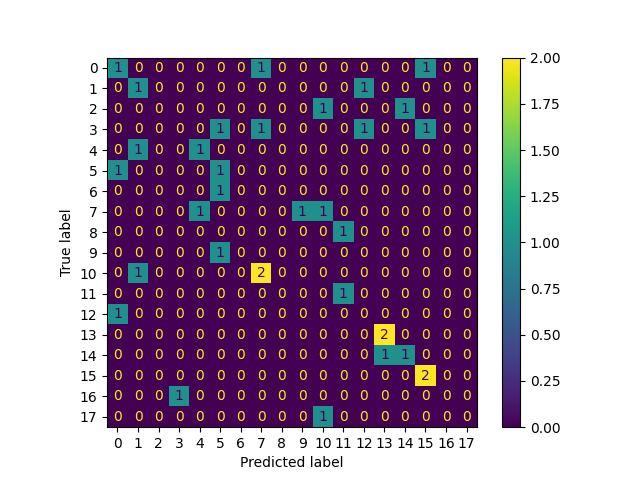
\includegraphics[width=0.45\textwidth]{dados/figuras/resultados/matrizes-confusao/tamura-vistex-knn.png}}}
    \qquad
    \subfloat[\centering MST]{{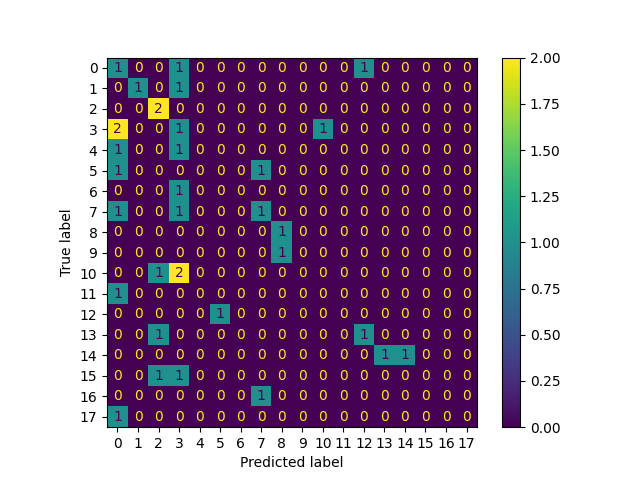
\includegraphics[width=0.45\textwidth]{dados/figuras/resultados/matrizes-confusao/mst-vistex-knn.png} }}
    \fonte{Autoria Própria.}
    \label{fig:vistexKNNMatrizConfusao}
\end{figure}

\begin{figure}[H]
    \centering
    \caption{Matrizes de confusão para o \textit{dataset} VisTex com uso de \textit{Linear} SVC}
    \subfloat[\centering LBP]{{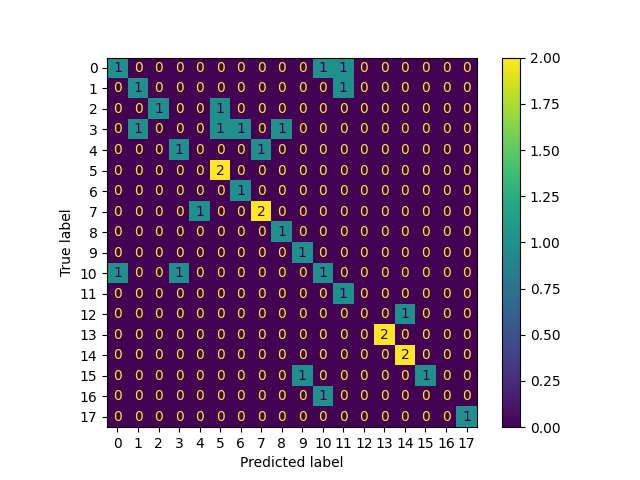
\includegraphics[width=0.45\textwidth]{dados/figuras/resultados/matrizes-confusao/lbp-vistex-linear-svc.png} }}
    \qquad
    \subfloat[\centering Tamura]{{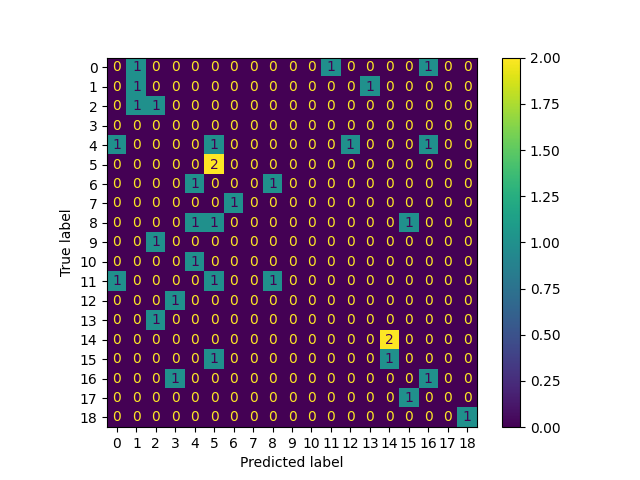
\includegraphics[width=0.45\textwidth]{dados/figuras/resultados/matrizes-confusao/tamura-vistex-linear-svc.png}}}
    \qquad
    \subfloat[\centering MST]{{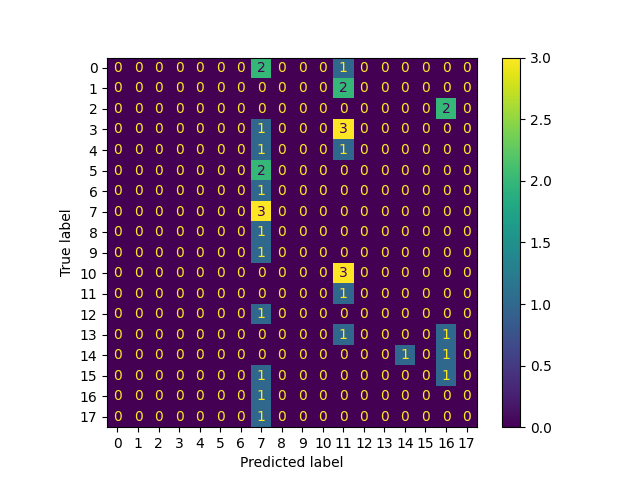
\includegraphics[width=0.45\textwidth]{dados/figuras/resultados/matrizes-confusao/mst-vistex-linear-svc.png}}}
    \fonte{Autoria Própria.}
    \label{fig:vistexLinearSVCMatrizConfusao}
\end{figure}

\begin{figure}[H]
    \centering
    \caption{Matrizes de confusão para o \textit{dataset} VisTex com uso de SVC}
    \subfloat[\centering Tamura]{{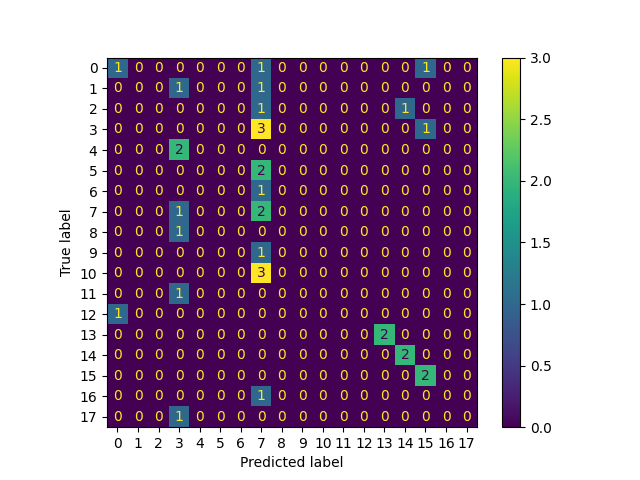
\includegraphics[width=0.45\textwidth]{dados/figuras/resultados/matrizes-confusao/tamura-vistex-svc.png} }}
    \qquad
    \subfloat[\centering Haralick]{{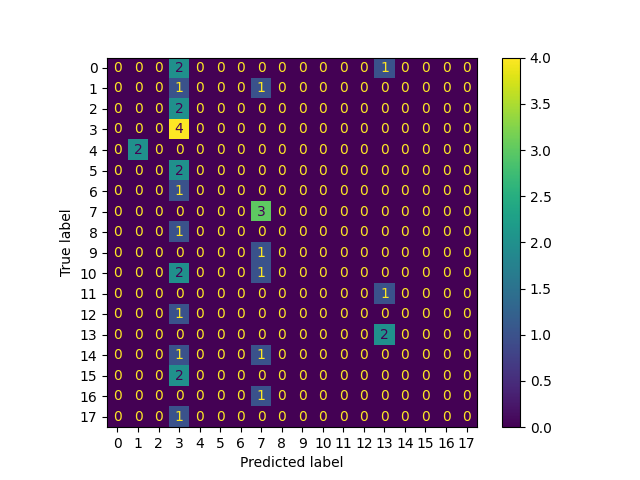
\includegraphics[width=0.45\textwidth]{dados/figuras/resultados/matrizes-confusao/haralick-vistex-svc.png}}}
    \qquad
    \subfloat[\centering Gabor]{{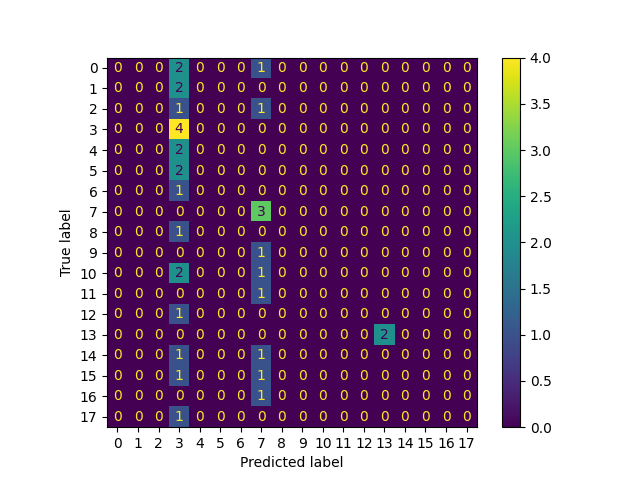
\includegraphics[width=0.45\textwidth]{dados/figuras/resultados/matrizes-confusao/gabor-vistex-svc.png}}}
    \qquad
    \subfloat[\centering MST]{{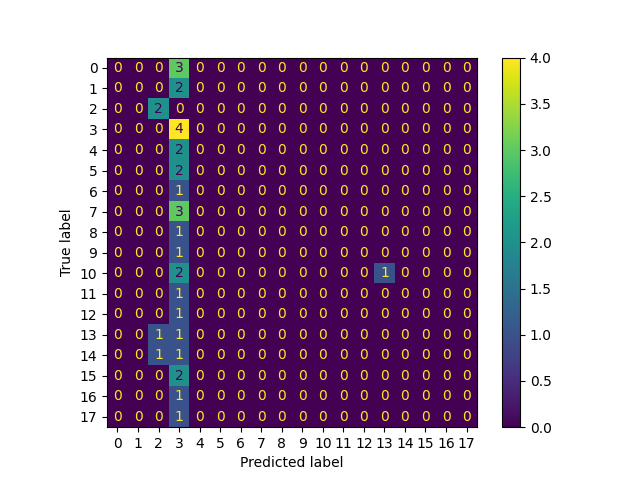
\includegraphics[width=0.45\textwidth]{dados/figuras/resultados/matrizes-confusao/mst-vistex-svc.png}}}
    \fonte{Autoria Própria.}
    \label{fig:vistexSVCMatrizConfusao}
\end{figure}
